\documentclass{standalone}
\usepackage{tikz}
\usepackage{ctex,siunitx}
\setCJKmainfont{Noto Serif CJK SC}
\usepackage{tkz-euclide}
\usepackage{amsmath}
\usetikzlibrary{patterns, calc,3d}
\usetikzlibrary {decorations.pathmorphing,decorations.pathreplacing,decorations.shapes}
\tikzset{label style/.append style={font=\small}}
\begin{document}
\small
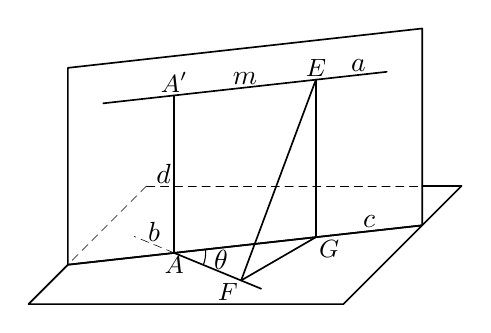
\begin{tikzpicture}[>=latex,scale=1.0,inner sep=1pt]
  \tkzDefPoints{0/0/M,4/0/N,5.5/1.5/P,1.5/1.5/Q,0.5/0.5/R,5/1.0/S,5/3.5/T,0.5/3/U,2.7/0.3/F}
  \tkzDefPointOnLine[pos=0.3](R,S)\tkzGetPoint{A}
  \tkzDefPointOnLine[pos=0.7](R,S)\tkzGetPoint{G}
  \tkzDefShiftPoint[A](0,2){A'}
  \tkzDefShiftPoint[G](0,2){E}
  \tkzInterLL(P,Q)(S,T)\tkzGetPoint{S'}
  \tkzDrawPolygon[semithick](M,N,S,R)
  \tkzDrawPolygon[semithick](R,S,T,U)
  \tkzDrawSegments[semithick](S',P P,S E,G F,G E,F A,A')
  \tkzDrawLine[add=0.5 and 0.5,semithick](A',E)
  \tkzDrawLine[add =0 and 0.3,semithick](A,F)
  \tkzDrawLine[add =-1 and 0.6,densely dashed](F,A)
  \tkzDrawSegments[densely dashed](Q,R Q,S')
  \tkzLabelLine[pos=0.5,left](A,A'){$d$}
  \tkzLabelLine[pos=1.3,above](F,A){$b$}
  \tkzLabelLine[pos=0.5,above](E,A'){$m$}
  \tkzLabelLine[pos=0.5,above](G,S){$c$}
  \tkzLabelLine[pos=1.3,above](A',E){$a$}
  \tkzLabelPoints[above](A',E)
  \tkzLabelPoints[below right](G)
  \tkzLabelPoints[below left](F)
  \tkzLabelPoints(A)
  \tkzMarkAngle[size=0.4](F,A,G)
  \tkzLabelAngle[pos=0.6](F,A,G){$\theta$}
\end{tikzpicture}
\end{document}